%%%%%%%%%%%%%%%%%%%%%%%%%%%%%%%%%%%%%%%%%
% Beamer Presentation
% LaTeX Template
% Version 1.0 (10/11/12)
%
% This template has been downloaded from:
% http://www.LaTeXTemplates.com
%
% License:
% CC BY-NC-SA 3.0 (http://creativecommons.org/licenses/by-nc-sa/3.0/)
%
% Modified by Jeremie Gillet in November 2015 to make an OIST Skill Pill template
%
%%%%%%%%%%%%%%%%%%%%%%%%%%%%%%%%%%%%%%%%%

%-------------------------------------------------------------------------------
%	PACKAGES AND THEMES
%-------------------------------------------------------------------------------

\documentclass{beamer}

\mode<presentation> {

\usetheme{Madrid}

\definecolor{OISTcolor}{rgb}{0.65,0.16,0.16}
\usecolortheme[named=OISTcolor]{structure}

%\setbeamertemplate{footline} % To remove the footer line in all slides uncomment this line
%\setbeamertemplate{footline}[page number] % To replace the footer line in all slides with a simple slide count uncomment this line

\setbeamertemplate{navigation symbols}{} % To remove the navigation symbols from the bottom of all slides uncomment this line
}
\setbeamertemplate{itemize items}[triangle]
\setbeamertemplate{enumerate items}[default]

\usepackage{graphicx} % Allows including images
\usepackage{booktabs} % Allows the use of \toprule, \midrule and \bottomrule in tables
\usepackage{textpos} % Use for positioning the Skill Pill logo
\usepackage{fancyvrb}
\usepackage{tikz}
\usepackage{hyperref}
\usepackage{listings}

\definecolor{dkgreen}{rgb}{0,0.6,0}
\definecolor{gray}{rgb}{0.5,0.5,0.5}
\definecolor{mauve}{rgb}{0.58,0,0.82}

\lstset{frame=tb,
  language=python,
  aboveskip=3mm,
  belowskip=3mm,
  showstringspaces=false,
  columns=flexible,
  basicstyle={\small\ttfamily},
  numbers=none,
  numberstyle=\tiny\color{gray},
  keywordstyle=\color{blue},
  commentstyle=\color{dkgreen},
  stringstyle=\color{mauve},
  breaklines=true,
  breakatwhitespace=true,
  tabsize=3
}

%-------------------------------------------------------------------------------
%	TITLE PAGE
%-------------------------------------------------------------------------------

\title[Intro.jl]{Introduction to Julia} % The short title appears at the bottom of every slide, the full title is only on the title page
\subtitle{Session 1: Introduction}

\author{James Schloss} % Your name
\institute[LeiosLabs] % Your institution as it will appear on the bottom of every slide, may be shorthand to save space
{
\textit{jrs.schloss@gmail.com} % Your email address
}
\date{October 9, 2023} % Date, can be changed to a custom date

\begin{document}

\begin{frame}
\vspace*{1.4cm}
\titlepage % Print the title page as the first slide
\end{frame}

\setbeamertemplate{background}{} % No background logo after title frame

\begin{frame}
\frametitle{Disclaimer}
\center \Huge{Ok, look.}
\end{frame}

\begin{frame}
\frametitle{Disclaimer}
\center \Huge{You can find everything I am about to show you online, but Julia documentation kinda sucks}
\center \small{I'm working on it kinda}
\end{frame}

\begin{frame}
\frametitle{Disclaimer}

\center My point here is to (hopefully) interest you and show you how Julia works.

\pause
\center Essentially, I want you to come off of this course with a deeper understanding of Julia than whatever language you typically use for development.
\end{frame}

\begin{frame}
\frametitle{What is Julia?}

\pause
\center \Huge{Simplicity $\neq$ Ease of use}

\end{frame}

\begin{frame}
\frametitle{What is Julia?}
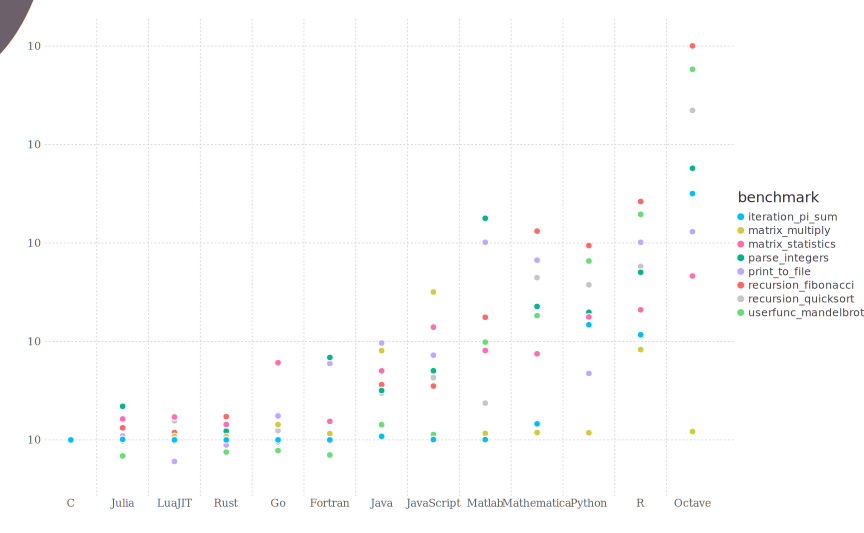
\includegraphics[width=\textwidth]{res/benchmarks.png}
\end{frame}

\begin{frame}
\frametitle{Let's test it out!}

\center \Huge{Python vs C vs Julia}
\center \small{Who will win in this epic showdown?}
\end{frame}

\begin{frame}
\frametitle{Introduction to the package management}
Here we will do the following:
\begin{enumerate}
\item Create a new package
\item Install a package
\item Describe what the Project.toml is
\item Talk about deps and compat bounds
\item Talk about the Manifest.toml
\item Talk about testing, building, etc
\end{enumerate}
\end{frame}

\begin{frame}
\frametitle{Development environments}

\begin{itemize}
\item Text Editor + REPL
\item Pluto.jl
\item VSCode
\end{itemize}

\end{frame}

\begin{frame}
\frametitle{An intro to Julia syntax}
\center yeah...
\end{frame}

\begin{frame}
\frametitle{An intro to Julia syntax}
\center We're doing an Nbody sim
\end{frame}

\begin{frame}
\frametitle{An intro to Julia syntax}
\center It's simple and builds into the topic discussions for next time
\end{frame}

\begin{frame}
\frametitle{Bits and Bobs...}
\begin{itemize}
\item Multiple dispatch
\item Types and supertypes
\item Broadcasting
\item Unicode
\item PkgCompiler
\end{itemize}
\end{frame}

\end{document}
